\documentclass[]{beamer}
\usepackage[T1]{fontenc}
\usepackage[utf8]{inputenc}
\usepackage{lmodern}
\usepackage[italian]{babel}
\usepackage{mathrsfs}
\usepackage{cancel}

\title{La relatività generale}
\author{\texorpdfstring{Mattia Cozzi\newline\href{mailto:cozzimattia@gmail.com}{\texttt{cozzimattia@gmail.com}}}{Mattia Cozzi}}
\date{a.s.~2023/2024}

%\documentclass[handout]{beamer}     %usare questa classe per generare l'handout
%\usepackage{pgfpages}   %per mostrare più quadri nella stessa pagina
%\pgfpagesuselayout{4 on 1}[a4paper,border shrink=5mm,landscape]
\usetheme{Singapore}
%\useoutertheme[left]{sidebar} %elementi intorno alle diapositive
\setbeamercovered{dynamic} %modifica l'aspetto del testo grigetto delle diapositive future. Argomenti: invisible/transparent/dynamic
\usecolortheme{orchid}
%COLORE PRINCIPALE
% \definecolor{marroncino}{RGB}{156, 26, 0} % UBC Blue (primary)
% \setbeamercolor{structure}{fg=marroncino} % itemize, enumerate, etc


\theoremstyle{plain}
\newtheorem{teorema}{Teorema}

\usepackage{tikz}
\usepackage{circuitikz}


\usepackage{pgf,pgfplots,graphicx}
\usetikzlibrary{angles,quotes,arrows,shapes,decorations.markings}
\pgfplotsset{compat=1.15}
\usepgfplotslibrary{units,fillbetween} % to add units easily to axis
\tikzset{fleche/.style args={#1:#2}{postaction=decorate,decoration={name=markings,mark=at position #1 with {\arrow[#2,scale=2]{>}}},},}




\def\angolo[#1](#2)(#3:#4:#5)% Syntax: [draw options] (center) (initial angle:final angle:radius)
    { \draw[#1] ($(#2)+({#5*cos(#3)},{#5*sin(#3)})$) arc (#3:#4:#5); }



\begin{document}

\begin{frame}
  \titlepage
\end{frame}





\begin{frame}
\frametitle{Contenuti}
\tableofcontents
\end{frame}

\section{Masse}

\begin{frame}
\frametitle{Massa gravitazionale e massa inerziale}
La massa gravitazionale di un corpo e la sua massa inerziale sono grandezze che hanno definizioni operative diverse, e sono pertanto logicamente distinte.\pause

\begin{columns}
\begin{column}{0.5\textwidth}
\begin{center}
Massa gravitazionale
\end{center}
\end{column}
\begin{column}{0.5\textwidth}
\begin{center}
Massa inerziale

\end{center}
\end{column}
\end{columns}

\begin{columns}
\begin{column}{0.5\textwidth}
\begin{center}
$ F = G \dfrac{M_g m_g}{r^2} $
\end{center}
\end{column}
\begin{column}{0.5\textwidth}
\begin{center}
$ F = m_i a $
\end{center}
\end{column}
\end{columns}

~

~

{\pause}Se proviamo a calcolare l'accelerazione di gravità $ g $ in un punto del pianeta, notiamo che essa dipende dal rapporto $ \frac{m_g}{m_i} $.\pause


~

Anche le più precise esperienze (ordine $ 10^{-14} $) mostrano tuttavia che la massa inerziale è equivalente alla massa gravitazionale.
\end{frame}


\section{Principi}

\begin{frame}
\frametitle{Equivalenza tra massa inerziale e gravitazionale}
Einstein nel suo lavoro del 1916, \emph{Die Grundlage der allgemeinen Relativit\"{a}tstheorie}, postula l'equivalenza tra le due masse.\pause

~

Per quanto banale possa sembrare, questo permette ad Einstein di formulare, proponendo anche alcuni esperimenti ideali, il:

~

\begin{block}{Principio di equivalenza}
In una zona limitata dello spaziotempo è sempre possibile scegliere un SDR in modo da simulare l'esistenza di un dato campo gravitazionale uniforme o, al contrario, in modo da eliminare l'effetto di una forza di gravità costante.
\end{block}
\end{frame}


\begin{frame}
\frametitle{Il principio di relatività generale}
Sappiamo che il principio di relatività ristretta afferma che ``le leggi e i principi della fisica hanno la stessa forma in tutti i sistemi di riferimento inerziali''.\pause

~

Avendo tuttavia posto equivalenti la massa inerziale e quella gravitazionale, non abbiamo più nessun reale motivo per ritenere ``privilegiati'' i SDR inerziali.\pause

~

\begin{block}{Principio di relatività generale}
Le leggi e i principi della fisica hanno la stessa forma in tutti i sistemi di riferimento.
\end{block}
\end{frame}

\section{Curvatura}

\begin{frame}
\frametitle{Conseguenze dei principi di Einstein}
I principi di Einstein comportano che anche la luce debba seguire le leggi della meccanica.\pause

\begin{figure}
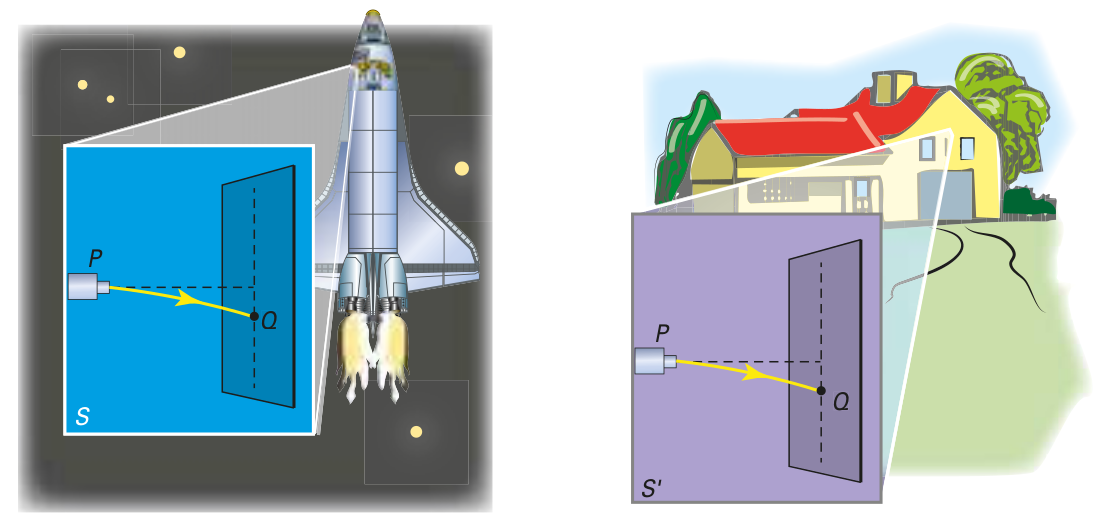
\includegraphics[width=.6\columnwidth]{img/relativitagen.png}
\end{figure}

Così come in un sistema accelerato un raggio luminoso segue una traiettoria curva, anche in presenza di un campo gravitazionale la luce dovrebbe seguire una traiettoria curva (le equazioni di Maxwell ne prevedono una rettilinea).
\end{frame}




\begin{frame}
\frametitle{Curvatura dello spaziotempo}
Il completo ripensamento della teoria della gravitazione richiese ad Einstein molti anni di lavoro, basandosi su due idee fondamentali:
\begin{itemize}
  \item lo \alert<1>{spaziotempo viene curvato dalla presenza di una massa}, con curvatura più accentuata più si è vicini ad essa;\pause
  \item \alert<2>{i corpi soggetti a gravità si muovono lungo le geodetiche} (curve di minima lunghezza) dello spaziotempo curvo.\pause
\end{itemize}

~

La relatività ristretta lavorava con uno spaziotempo a curvatura nulla, quella generale ne usa uno a curvatura positiva.
\begin{center}
\href{https://drive.google.com/open?id=1kI_uxzUEqqL2lPvsBEERMYCoG-gnTHZq}{\beamergotobutton{Geometrie non euclidee}}
\end{center}
\end{frame}

\begin{frame}
\frametitle{Gravitazione e inerzia come proprietà geometriche}
Nel modello della relatività generale la gravità non è più una forza ma una \alert{proprietà geometrica dello spaziotempo} che dipende dalla presenza di una massa.

~
\begin{flushright}

\begin{quote}
Spacetime tells matter how to move

matter tells spacetime how to curve.  
\end{quote}
John A.~Wheeler

\emph{Gravitation}, 1973
\end{flushright}
\end{frame}



\begin{frame}
  \frametitle{Gravitazione secondo Newton e secondo Einstein}
  \begin{columns}
    \begin{column}{0.3\textwidth}
      \begin{figure}
        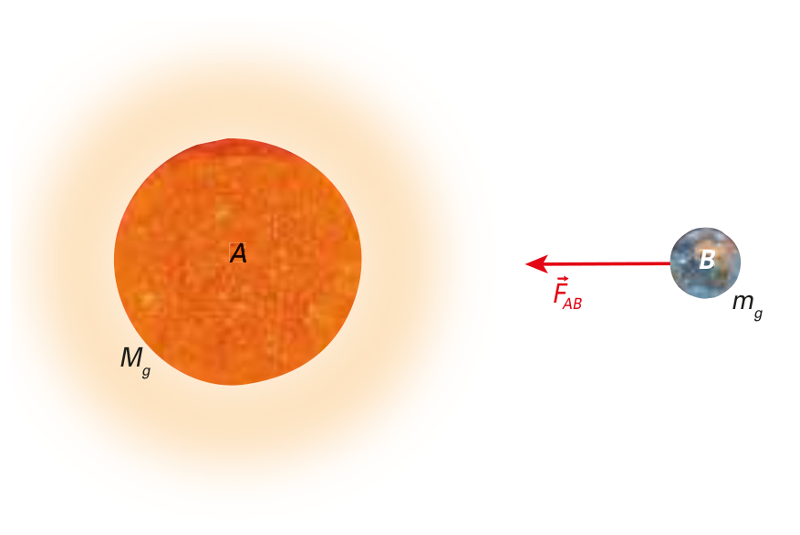
\includegraphics[width=\columnwidth]{img/gravity1.png}
      \end{figure}
    \end{column}
    \begin{column}{0.3\textwidth}
      \begin{figure}
        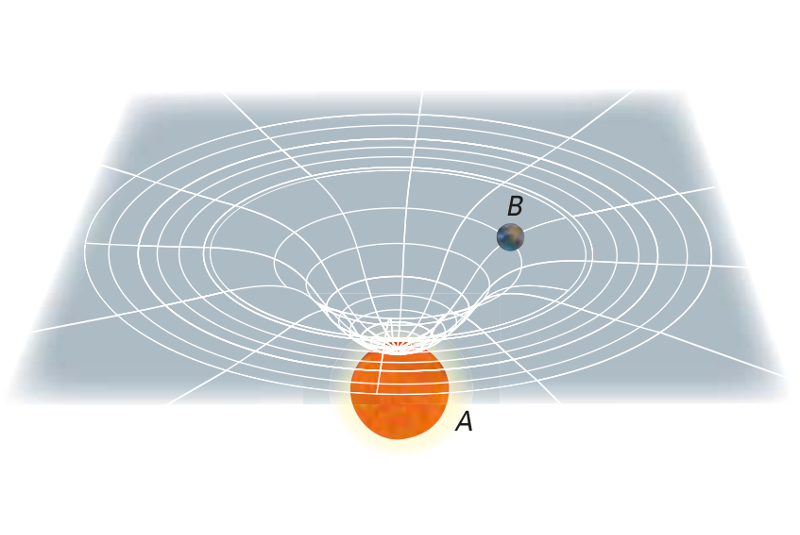
\includegraphics[width=\columnwidth]{img/gravity2.png}
      \end{figure}
    \end{column}
    \begin{column}{0.3\textwidth}
      \begin{figure}
        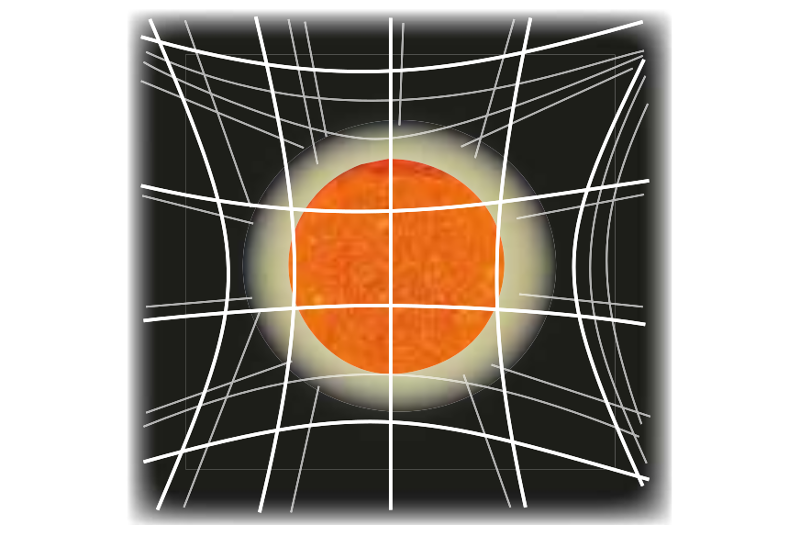
\includegraphics[width=\columnwidth]{img/gravity3.png}
      \end{figure}
    \end{column}

  \end{columns}
\end{frame}

\section{Luce}

\begin{frame}
\frametitle{Deflessione gravitazionale della luce}
La luce trasporta energia e, secondo la relatività ristretta, questa è equivalente ad una massa: $ m = \frac{E}{c^2} $.\pause

~

Ci aspettiamo pertanto degli effetti gravitazionali sulla luce (anche se la Terra non ha una massa sufficiente da renderli rilevabili).\pause

~

In effetti secondo la relatività generale la luce segue sempre le geodetiche e, se lo spazio viene curvato da una massa, essa seguirà una traiettoria curvilinea.
\end{frame}

\begin{frame}
\frametitle{Conferma sperimentale}
La prima conferma sperimentale si ebbe nel 1919 ad opera di Arthur Eddington, che misurò la posizione apparente di una stella tra durante un'eclissi di Sole, confrontandola con quella misurata con il Sole dalla parte opposta.
\begin{figure}
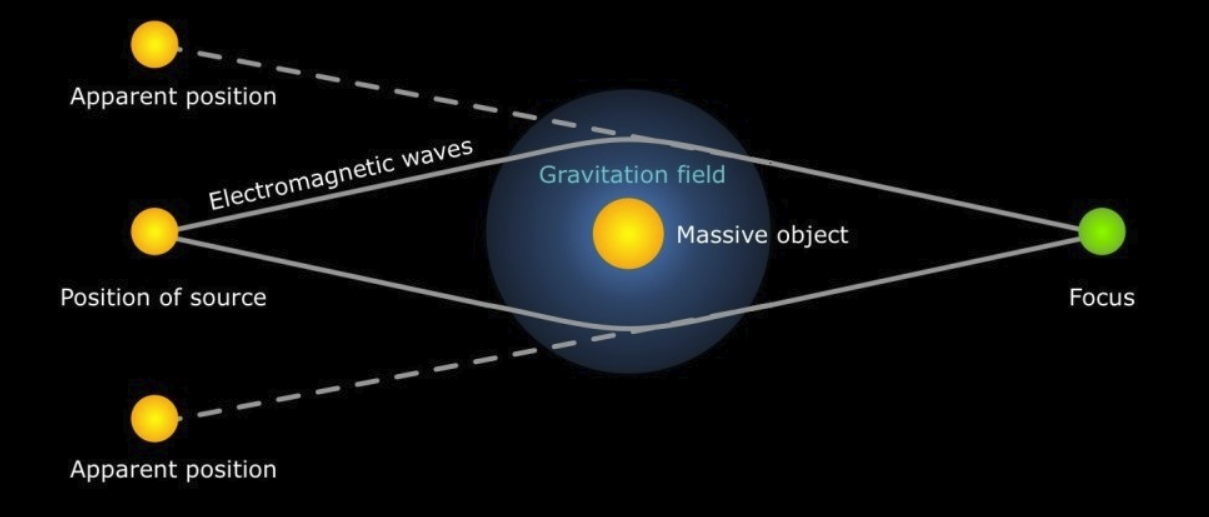
\includegraphics[width=.8\columnwidth]{img/deflessione.png}
\end{figure}

\end{frame}

\begin{frame}
\frametitle{Buchi neri}
Un buco nero è un oggetto celeste in cui una enorme quantità di materia è confinata in una porzione di spazio molto piccola.\pause

~

Per rendere la Terra un buco nero dovremmo comprimerla in una sfera di circa $ 9\, mm $ di raggio ($ r_T = 6400 \, km $).\pause

~

Il campo gravitazionale di un buco nero è così intenso che per sfuggirgli sarebbe necessaria una velocità di fuga superiore a $ c $.\pause

~

Quindi:
\begin{enumerate}
  \item un buco nero non è un buco, ma una massa;\pause
  \item i buchi neri non sono rilevabili direttamente, ma grazie ai loro effetti gravitazionali.
\end{enumerate}
\end{frame}

\begin{frame}
\frametitle{Onde gravitazionali}
La geometria dello spaziotempo della relatività generale dipende dalla distribuzione delle masse presenti.\pause

~

Se la distribuzione cambia (le masse si spostano) allora la geometria dello spaziotempo cambia.\pause

~

Tale variazione si propaga nell'Universo a velocità $ c $, generando una \alert{onda gravitazionale}.\pause

~

Tali onde, previste teoreticamente da Einstein nel 1916, sono state rilevate sperimentalmente per la prima volta l'11 febbraio 2016. Le onde rilevate erano state causate dalla collisione tra due buchi neri da 36 e 29 masse solari.
\begin{center}
\href{video/Ondegravitazionali.mp4}{\beamergotobutton{Video: Collisione tra due buchi neri}}
\end{center}
\end{frame}


\end{document}
